\subsection{How people cross an obstacle (Q1)}
\label{sec:res-biomech}

\subsubsection{Foot lift scales one-to-one with obstacle height}

Each participant lifts both feet almost exactly by the obstacle height (Figure~\ref{fig:strategy}). In the mixed model with a
random intercept and slope per participant (Table~\ref{tab:lme}), the leading foot rises by 10.1\,mm and the trailing foot by
11.1\,mm per cm of obstacle. The lift comes from 1.2\textdegree{} more leading-thigh flexion per cm and 1.2\textdegree{} more
backward tilt (heel-up) of the trailing shank per cm. The camera clearance margin does not change significantly with height:
people keep a nearly constant safety margin and simply raise the foot by the obstacle height.

\begin{figure}[htbp]
\centering
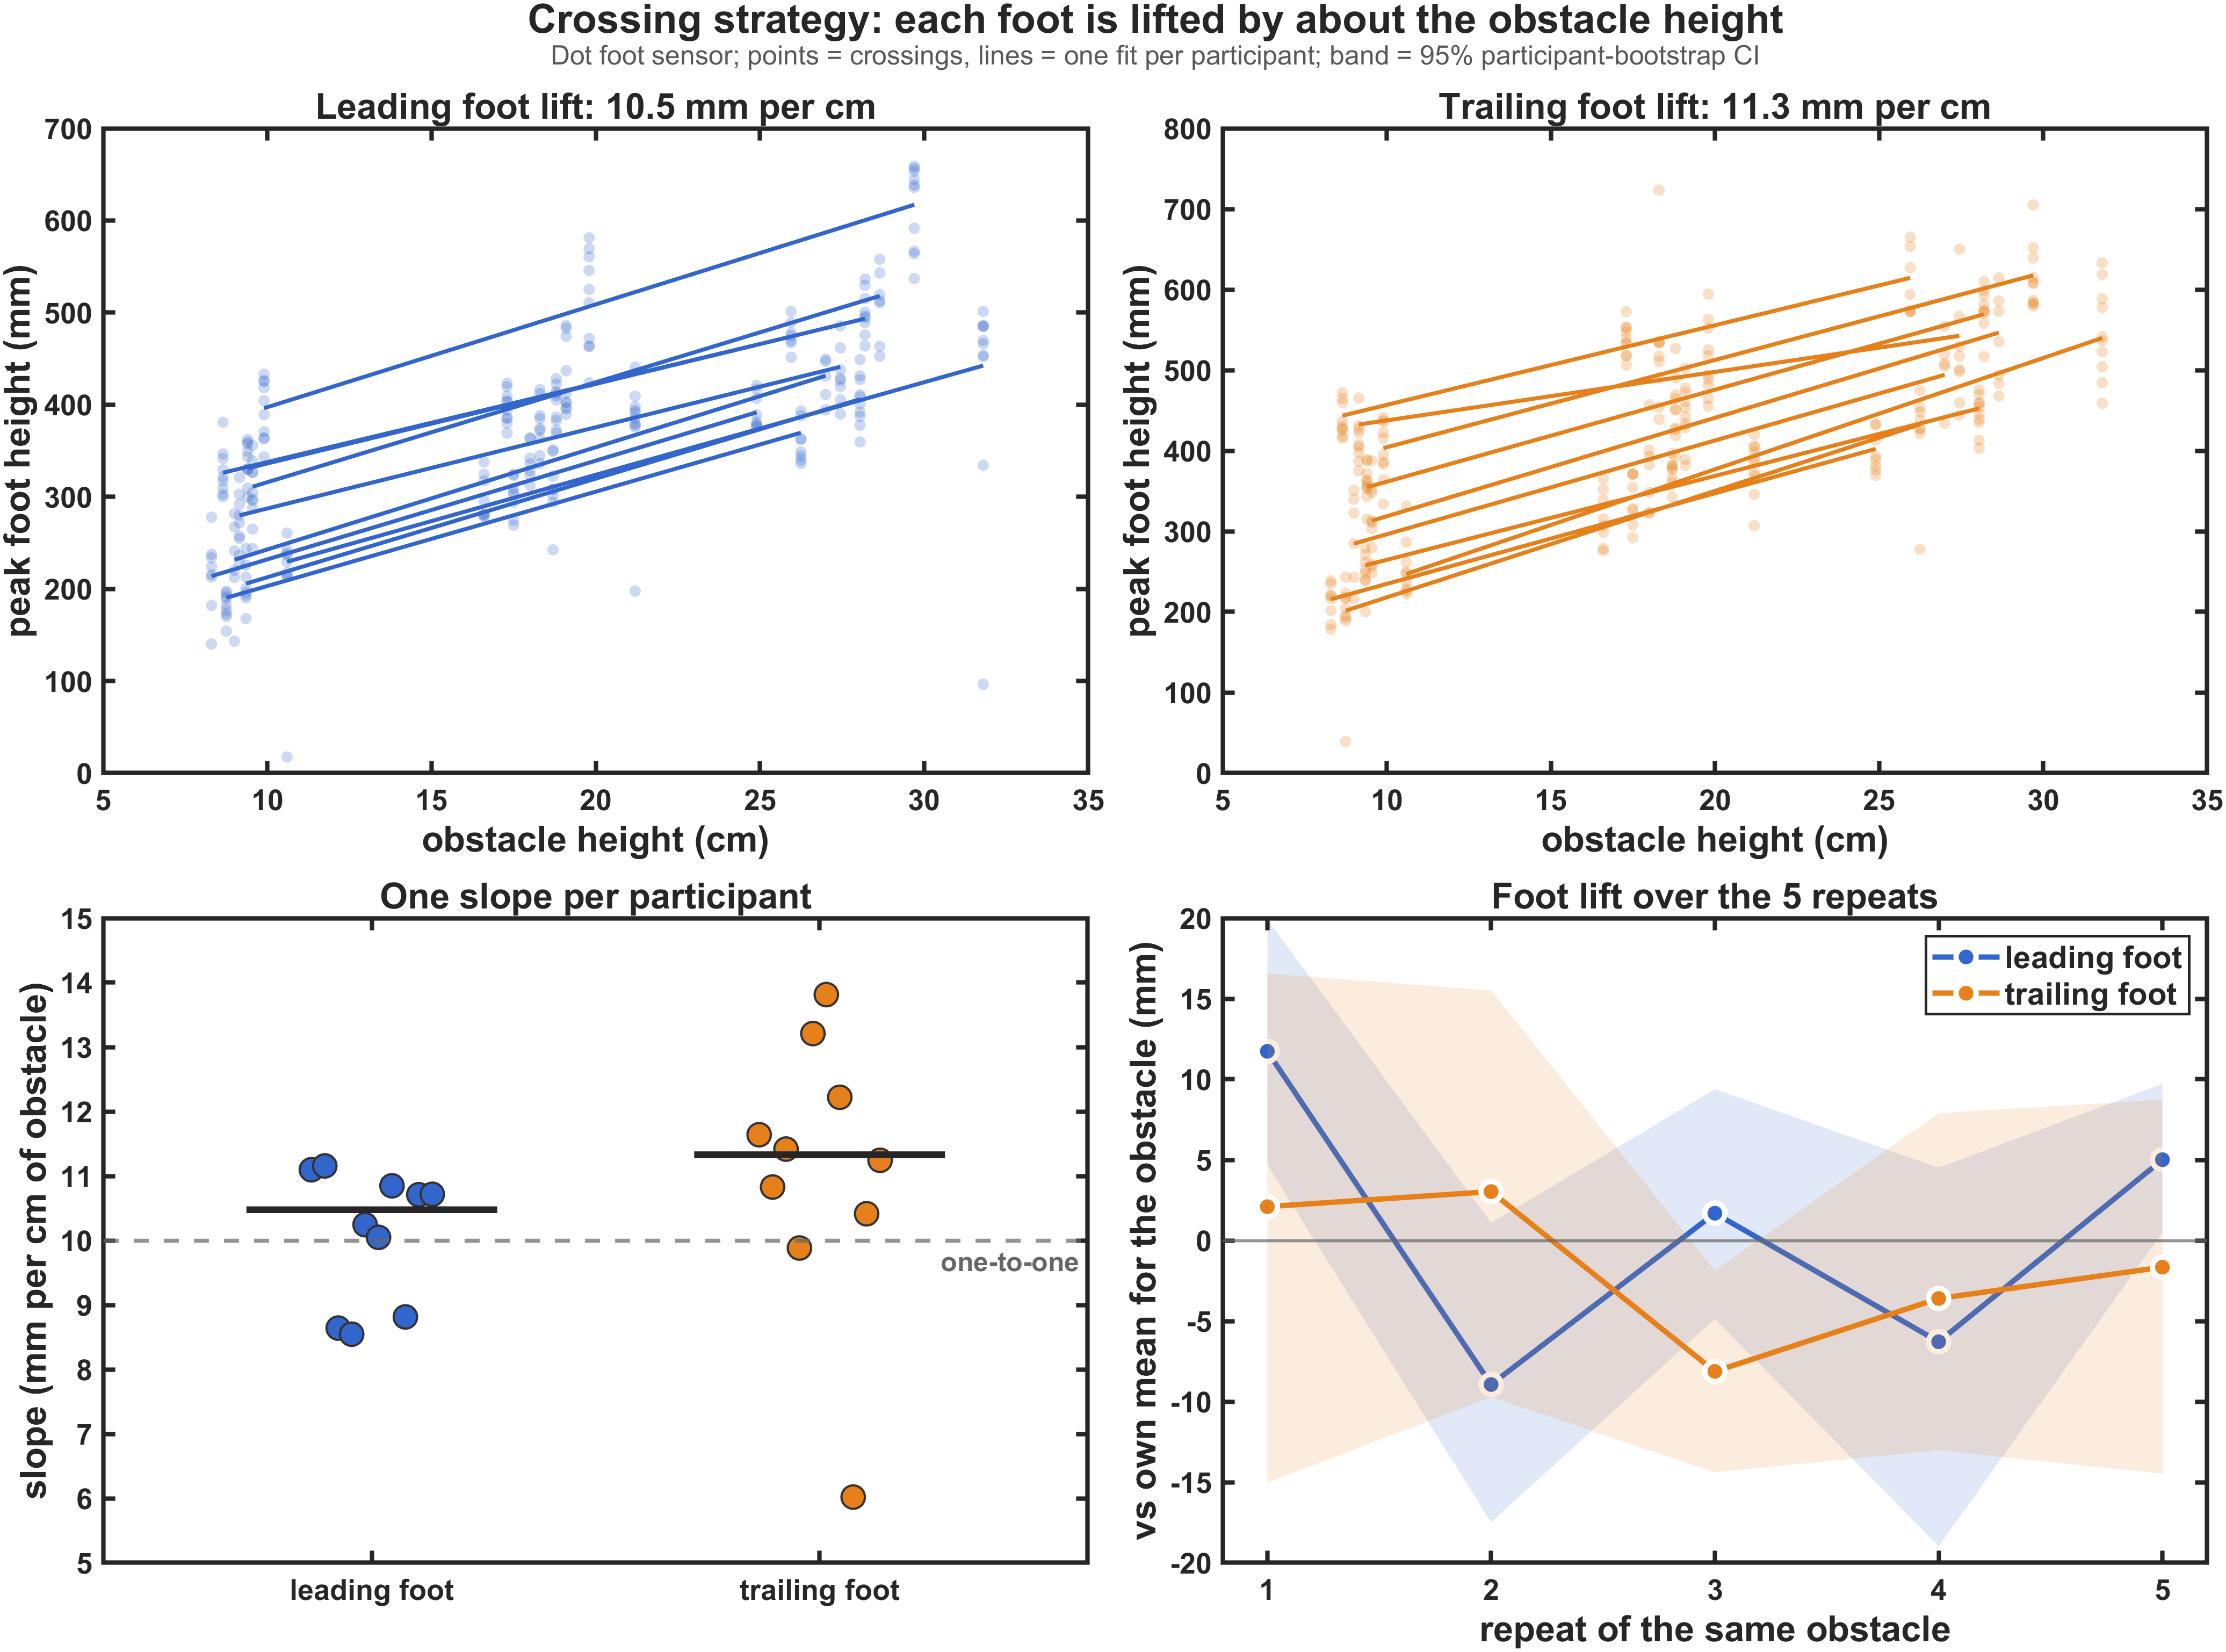
\includegraphics[width=\textwidth]{fig_story_strategy.png}
\caption{Crossing strategy. Top: foot lift measured by the Dot (foot-sensor rise above its stance height) against the nominal
obstacle height, leading (left) and trailing (right) foot; dots = crossings, one line per participant. Bottom left: the slope of each
participant (black bar = median; dashed = one-to-one, 10\,mm per cm). Bottom right: deviation of the foot lift from the participant
$\times$ obstacle mean over the five repeats of an obstacle (95\,\% CI). Source: \vn{crossing_ml_story.m}.}
\label{fig:strategy}
\end{figure}

\begin{table}[htbp]
\centering
\caption{Mixed-effects scaling with obstacle height: $y = \beta_0 + \beta_1 h + u_{0p} + u_{1p} h + \varepsilon$, slope $\beta_1$
per cm of obstacle (Satterthwaite CI and $p$).}
\label{tab:lme}
\begin{adjustbox}{max width=\textwidth}
{\footnotesize
\begin{tabular}{p{6cm}rrr}
\toprule
\textbf{variable} & \textbf{slope per cm} & \textbf{95\% CI} & \textbf{p} \\
\midrule
lead foot lift (Dot, mm) & +10.08 & +9.38 to +10.78 & $<$ 0.001 \\
trail foot lift (Dot, mm) & +11.12 & +9.66 to +12.59 & $<$ 0.001 \\
lead thigh flexion (deg) & +1.19 & +1.02 to +1.37 & $<$ 0.001 \\
trail shank backward tilt (deg) & $-$1.19 & $-$1.49 to $-$0.90 & $<$ 0.001 \\
lead min clearance (camera, mm) & $-$0.71 & $-$1.83 to +0.41 & 0.185 \\
trail min clearance (camera, mm) & $-$2.32 & $-$4.70 to +0.06 & 0.055 \\
\bottomrule
\end{tabular}
}
\end{adjustbox}

\end{table}

\paragraph{Adaptation over repeats.} The first crossing of a new obstacle has the highest leading-foot lift (+11.7\,mm above the
participant $\times$ obstacle mean, 95\,\% CI +4.7 to +19.9); later repeats scatter around the mean without a steady trend
(Figure~\ref{fig:strategy}, bottom right; Table~\ref{tab:adapt} in Appendix~\ref{app:extra}).

\subsubsection{Where and when the obstacle shows in the signals}

Figure~\ref{fig:map} shows, for every signal and every 2\,\% of the swing, the share of within-person variance explained by
height and by width ($\eta^2$). Table~\ref{tab:map} lists the peaks. Height is written most clearly in the trailing foot height
early in its swing ($\eta^2 = 0.76$ at 20\,\%), the trailing shank tilt at push-off (0.66 at 4\,\%), the leading foot height
around the apex (0.62 at 48\,\%) and the leading thigh tilt (0.47 at 60\,\%). The leading shank and leading foot tilt carry
little height information. Width never explains more than 8\,\% of any signal at any moment.

\begin{figure}[htbp]
\centering
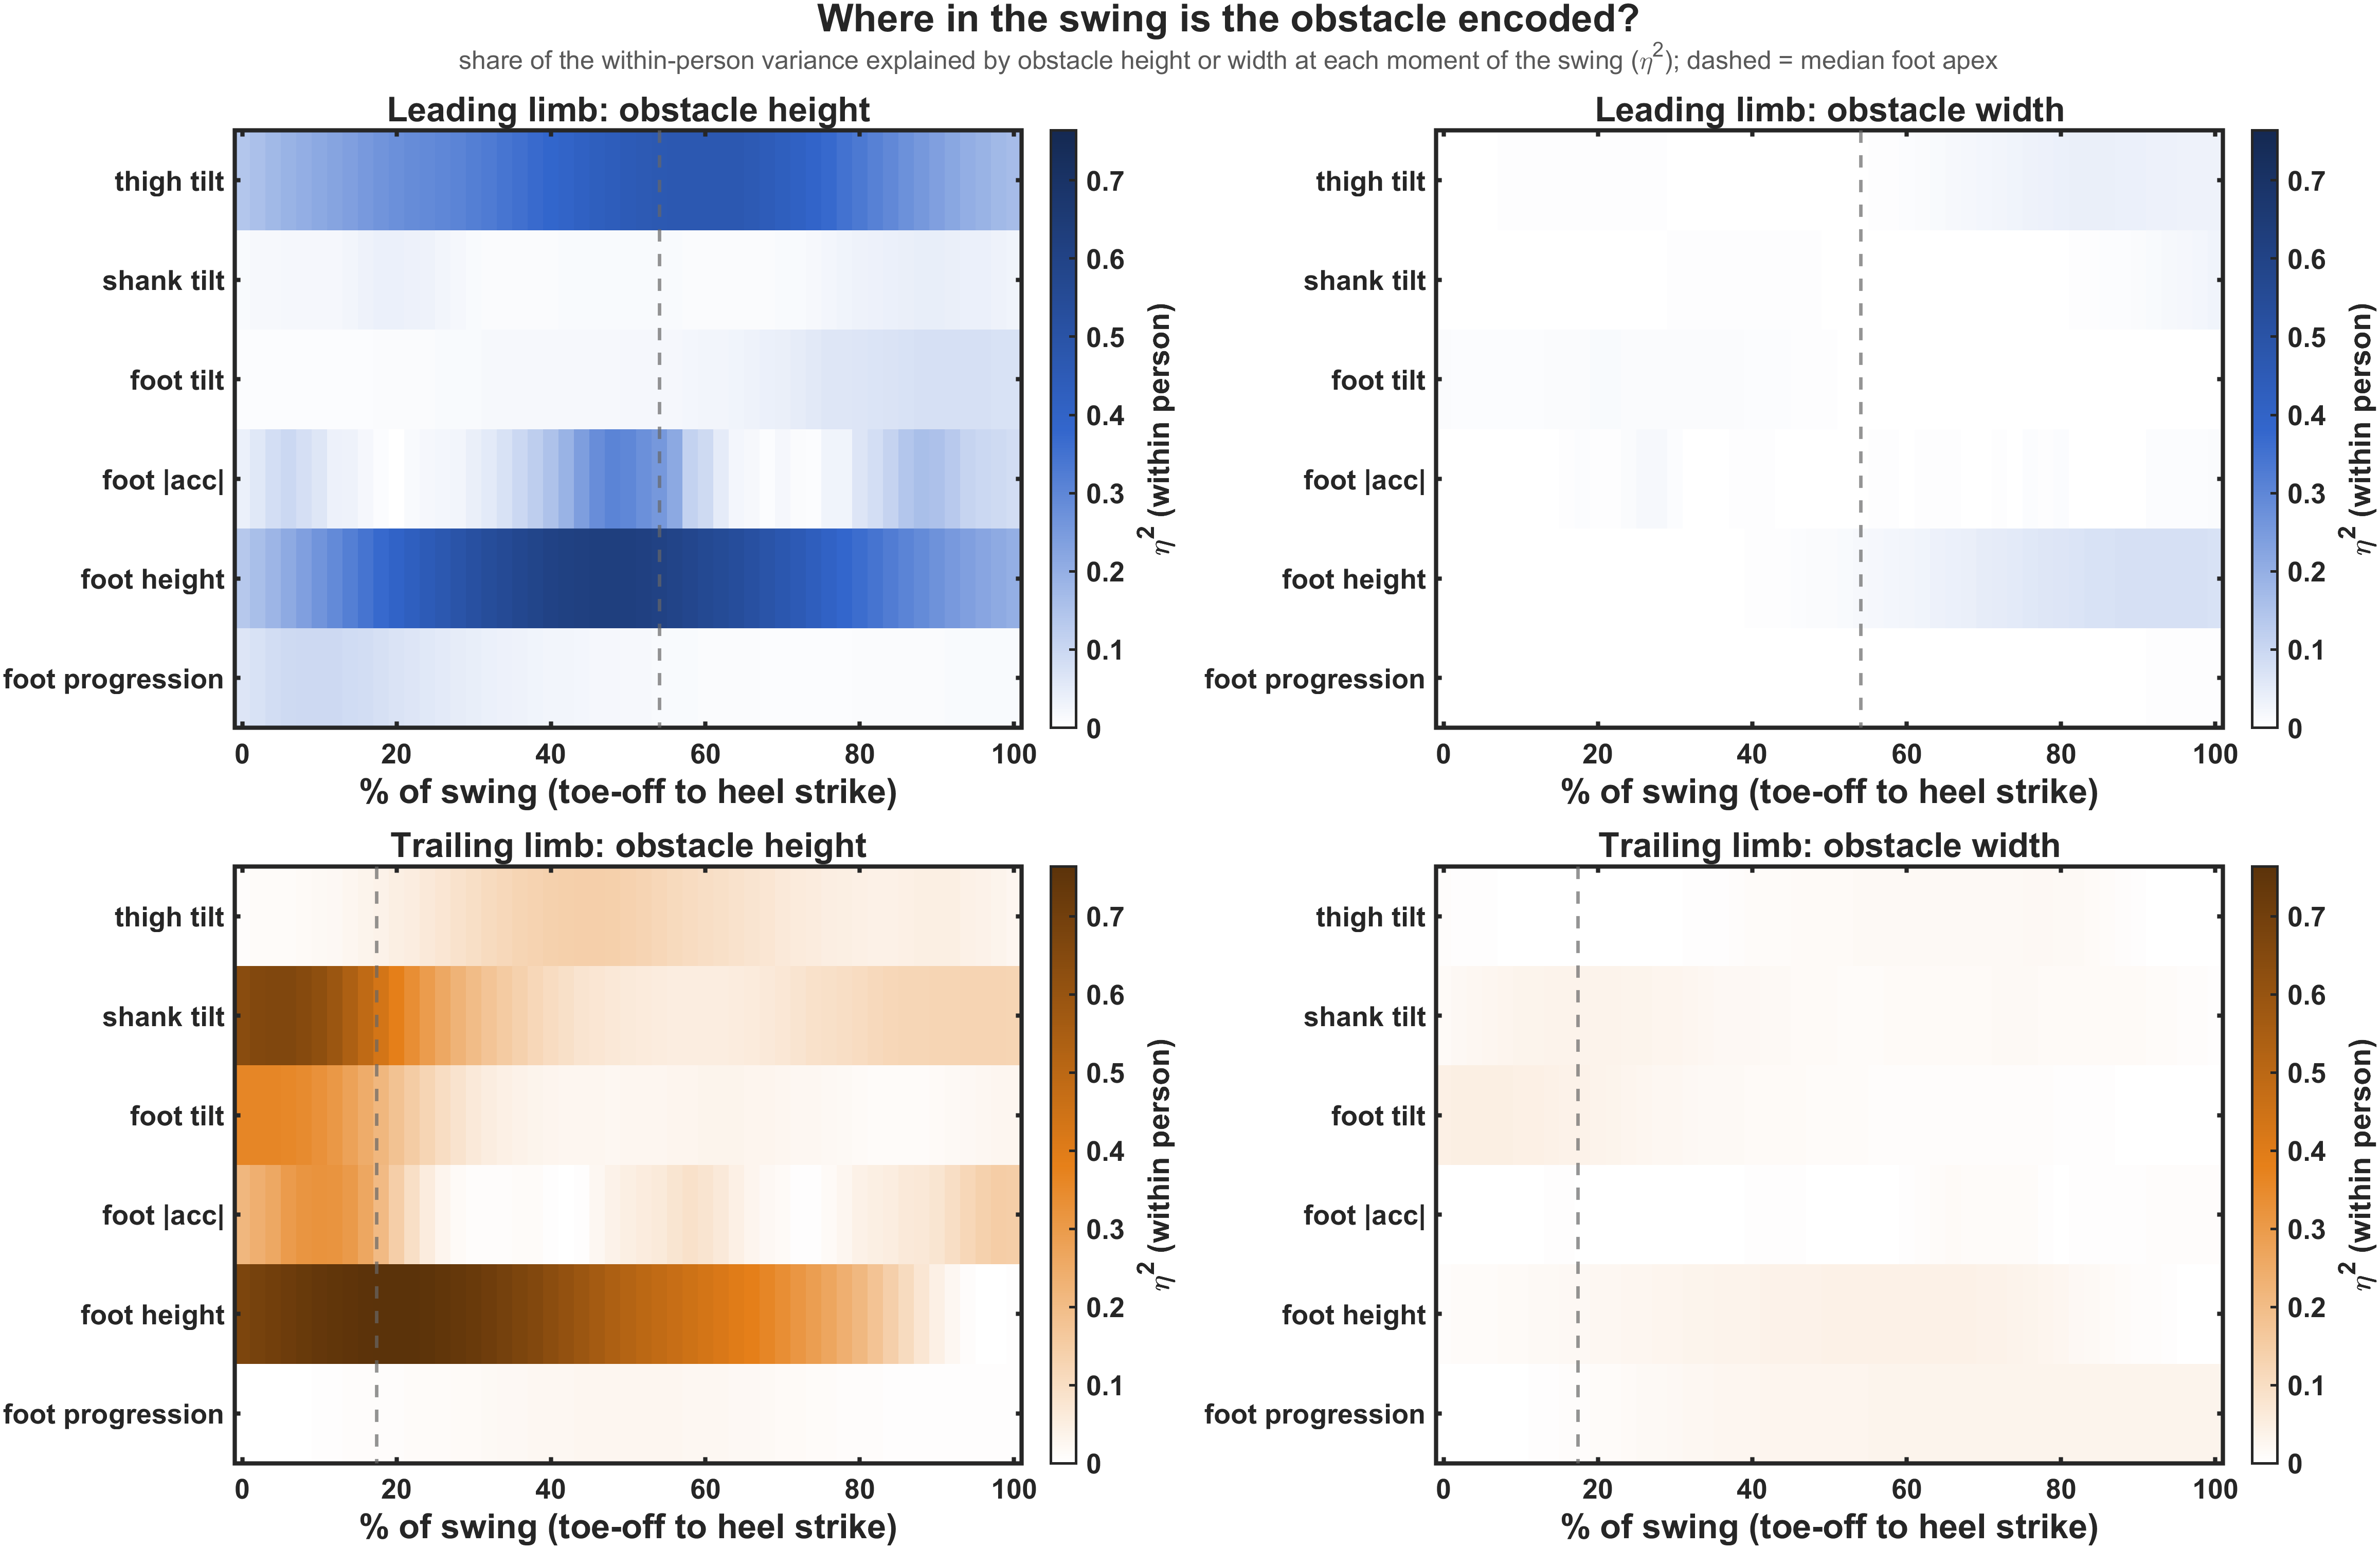
\includegraphics[width=\textwidth]{fig_story_map.png}
\caption{Within-person effect size $\eta^2$ of obstacle height (left) and width (right) at each moment of the swing, for the six
Dot swing signals of the leading (top, blue) and trailing (bottom, orange) limb, on the same scale. Dashed line = median foot apex.}
\label{fig:map}
\end{figure}

\begin{table}[htbp]
\centering
\caption{Peak $\eta^2$ of height and width per signal, and the share of variance explained by the participant (raw signals).}
\label{tab:map}
\begin{adjustbox}{max width=\textwidth}
{\footnotesize
\begin{tabular}{llrrrrr}
\toprule
\textbf{limb} & \textbf{signal} & \textbf{peak $\eta^2$ height} & \textbf{at \% swing} & \textbf{peak $\eta^2$ width} & \textbf{at \% swing} & \textbf{mean $\eta^2$ person (raw)} \\
\midrule
lead & thigh tilt & 0.47 & 60\% & 0.04 & 84\% & 0.40 \\
lead & shank tilt & 0.04 & 90\% & 0.03 & 100\% & 0.60 \\
lead & foot tilt & 0.08 & 90\% & 0.01 & 20\% & 0.46 \\
lead & foot |acc| & 0.31 & 48\% & 0.02 & 26\% & 0.32 \\
lead & foot height & 0.62 & 48\% & 0.08 & 92\% & 0.39 \\
lead & foot progression & 0.10 & 10\% & 0.01 & 100\% & 0.60 \\
trail & thigh tilt & 0.14 & 44\% & 0.02 & 76\% & 0.47 \\
trail & shank tilt & 0.66 & 4\% & 0.03 & 16\% & 0.40 \\
trail & foot tilt & 0.36 & 2\% & 0.05 & 6\% & 0.42 \\
trail & foot |acc| & 0.32 & 10\% & 0.01 & 66\% & 0.39 \\
trail & foot height & 0.76 & 20\% & 0.04 & 62\% & 0.48 \\
trail & foot progression & 0.03 & 50\% & 0.03 & 80\% & 0.71 \\
\bottomrule
\end{tabular}
}
\end{adjustbox}

\end{table}

\subsubsection{Every walker has a strong signature}

The participant explains far more variance than the obstacle: the median $\eta^2$ of the person over the 110 features is
0.42, that of height 0.02 (0.05 within person), and the person dominates in 99 of 110 features (Table~\ref{tab:person},
Figure~\ref{fig:person}). A logistic model identifies the participant from the features of a single crossing with 99.2\,\%
balanced accuracy (5-fold, chance 10\,\%). In a 2-D map of all crossings (t-SNE, Figure~\ref{fig:embed}) the raw features
cluster by participant (silhouette 0.48, by height $-0.04$); after person scaling they order by height (silhouette by height
0.26). This is the main reason why a model that has never seen the person is limited (Section~\ref{sec:res-height}).

\begin{table}[htbp]
\centering
\caption{Variance explained by the participant vs by the obstacle height (median over the 110 features).}
\label{tab:person}
\begin{adjustbox}{max width=\textwidth}
{\footnotesize
\begin{tabular}{p{5cm}rr}
\toprule
\textbf{} & \textbf{median over features} & \textbf{features where person $>$ height} \\
\midrule
$\eta^2$ person & 0.42 & 99 of 110 \\
$\eta^2$ height & 0.02 &  \\
$\eta^2$ height, within person & 0.05 &  \\
\bottomrule
\end{tabular}
}
\end{adjustbox}

\end{table}

\begin{figure}[htbp]
\centering
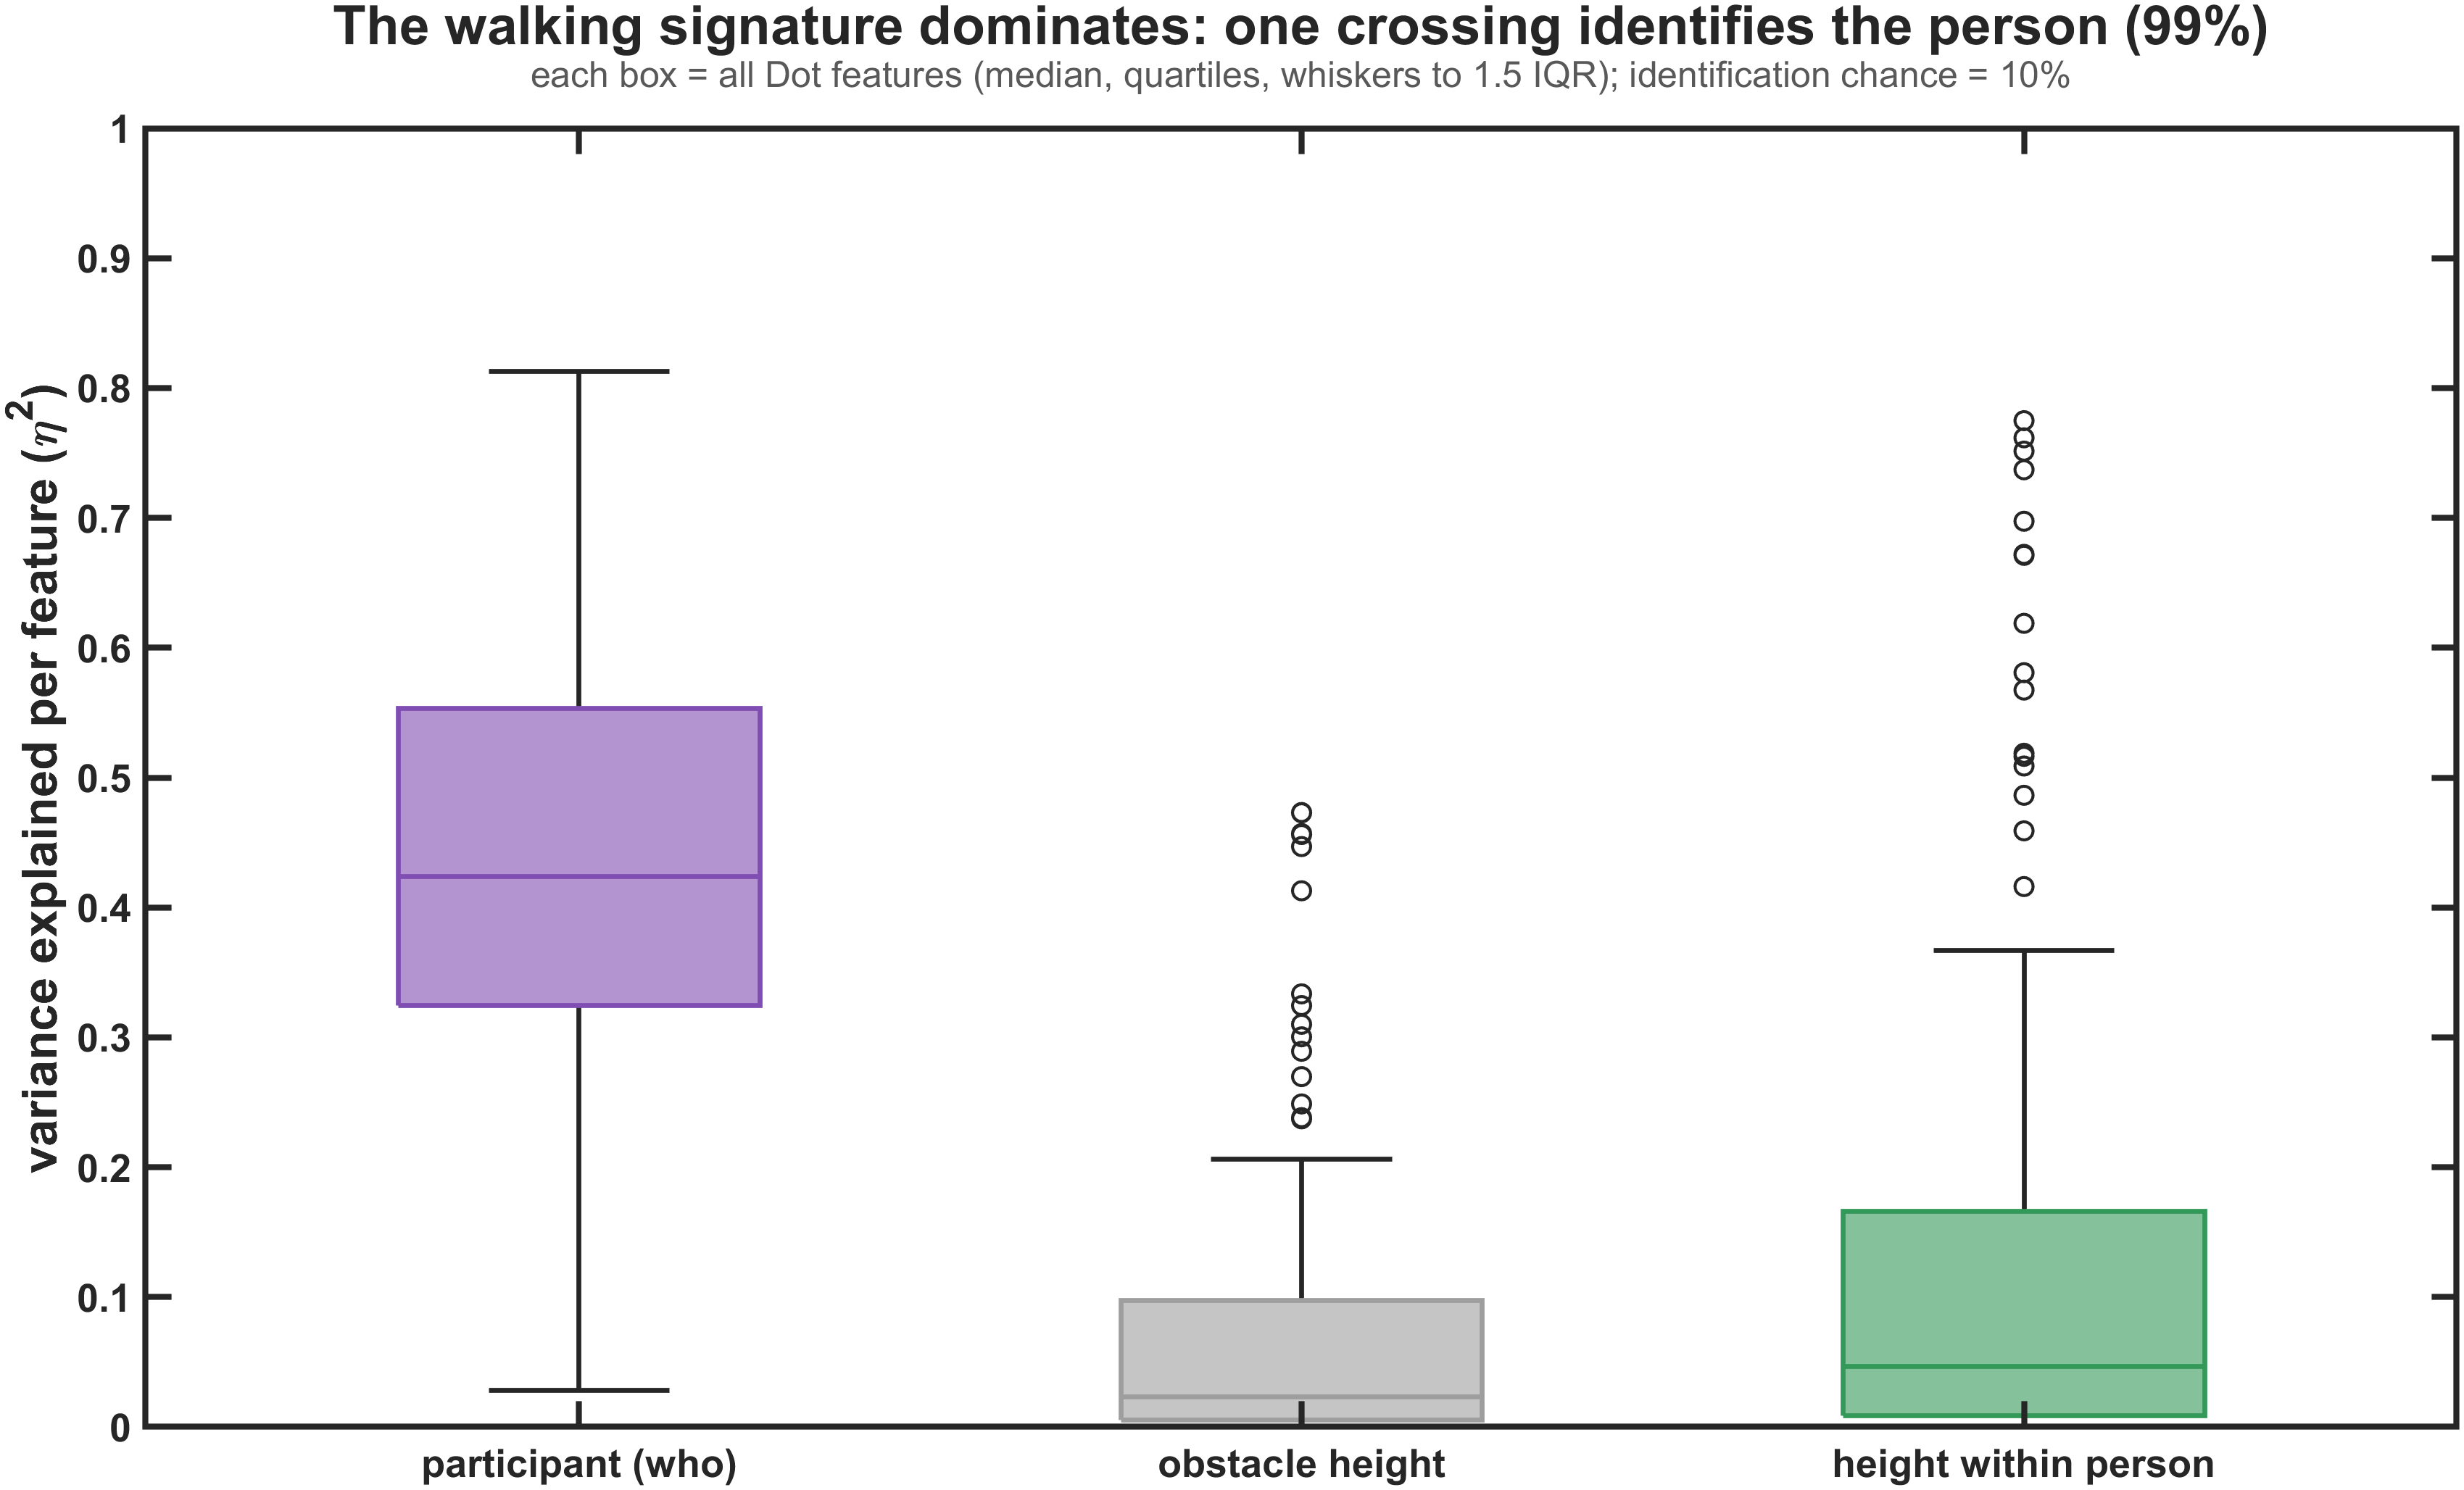
\includegraphics[width=0.78\textwidth]{fig_story_person.png}
\caption{Variance explained per feature by the participant (purple), by the obstacle height (grey), and by the height within each
participant (green); box = median and quartiles over the Dot features.}
\label{fig:person}
\end{figure}

\begin{figure}[htbp]
\centering
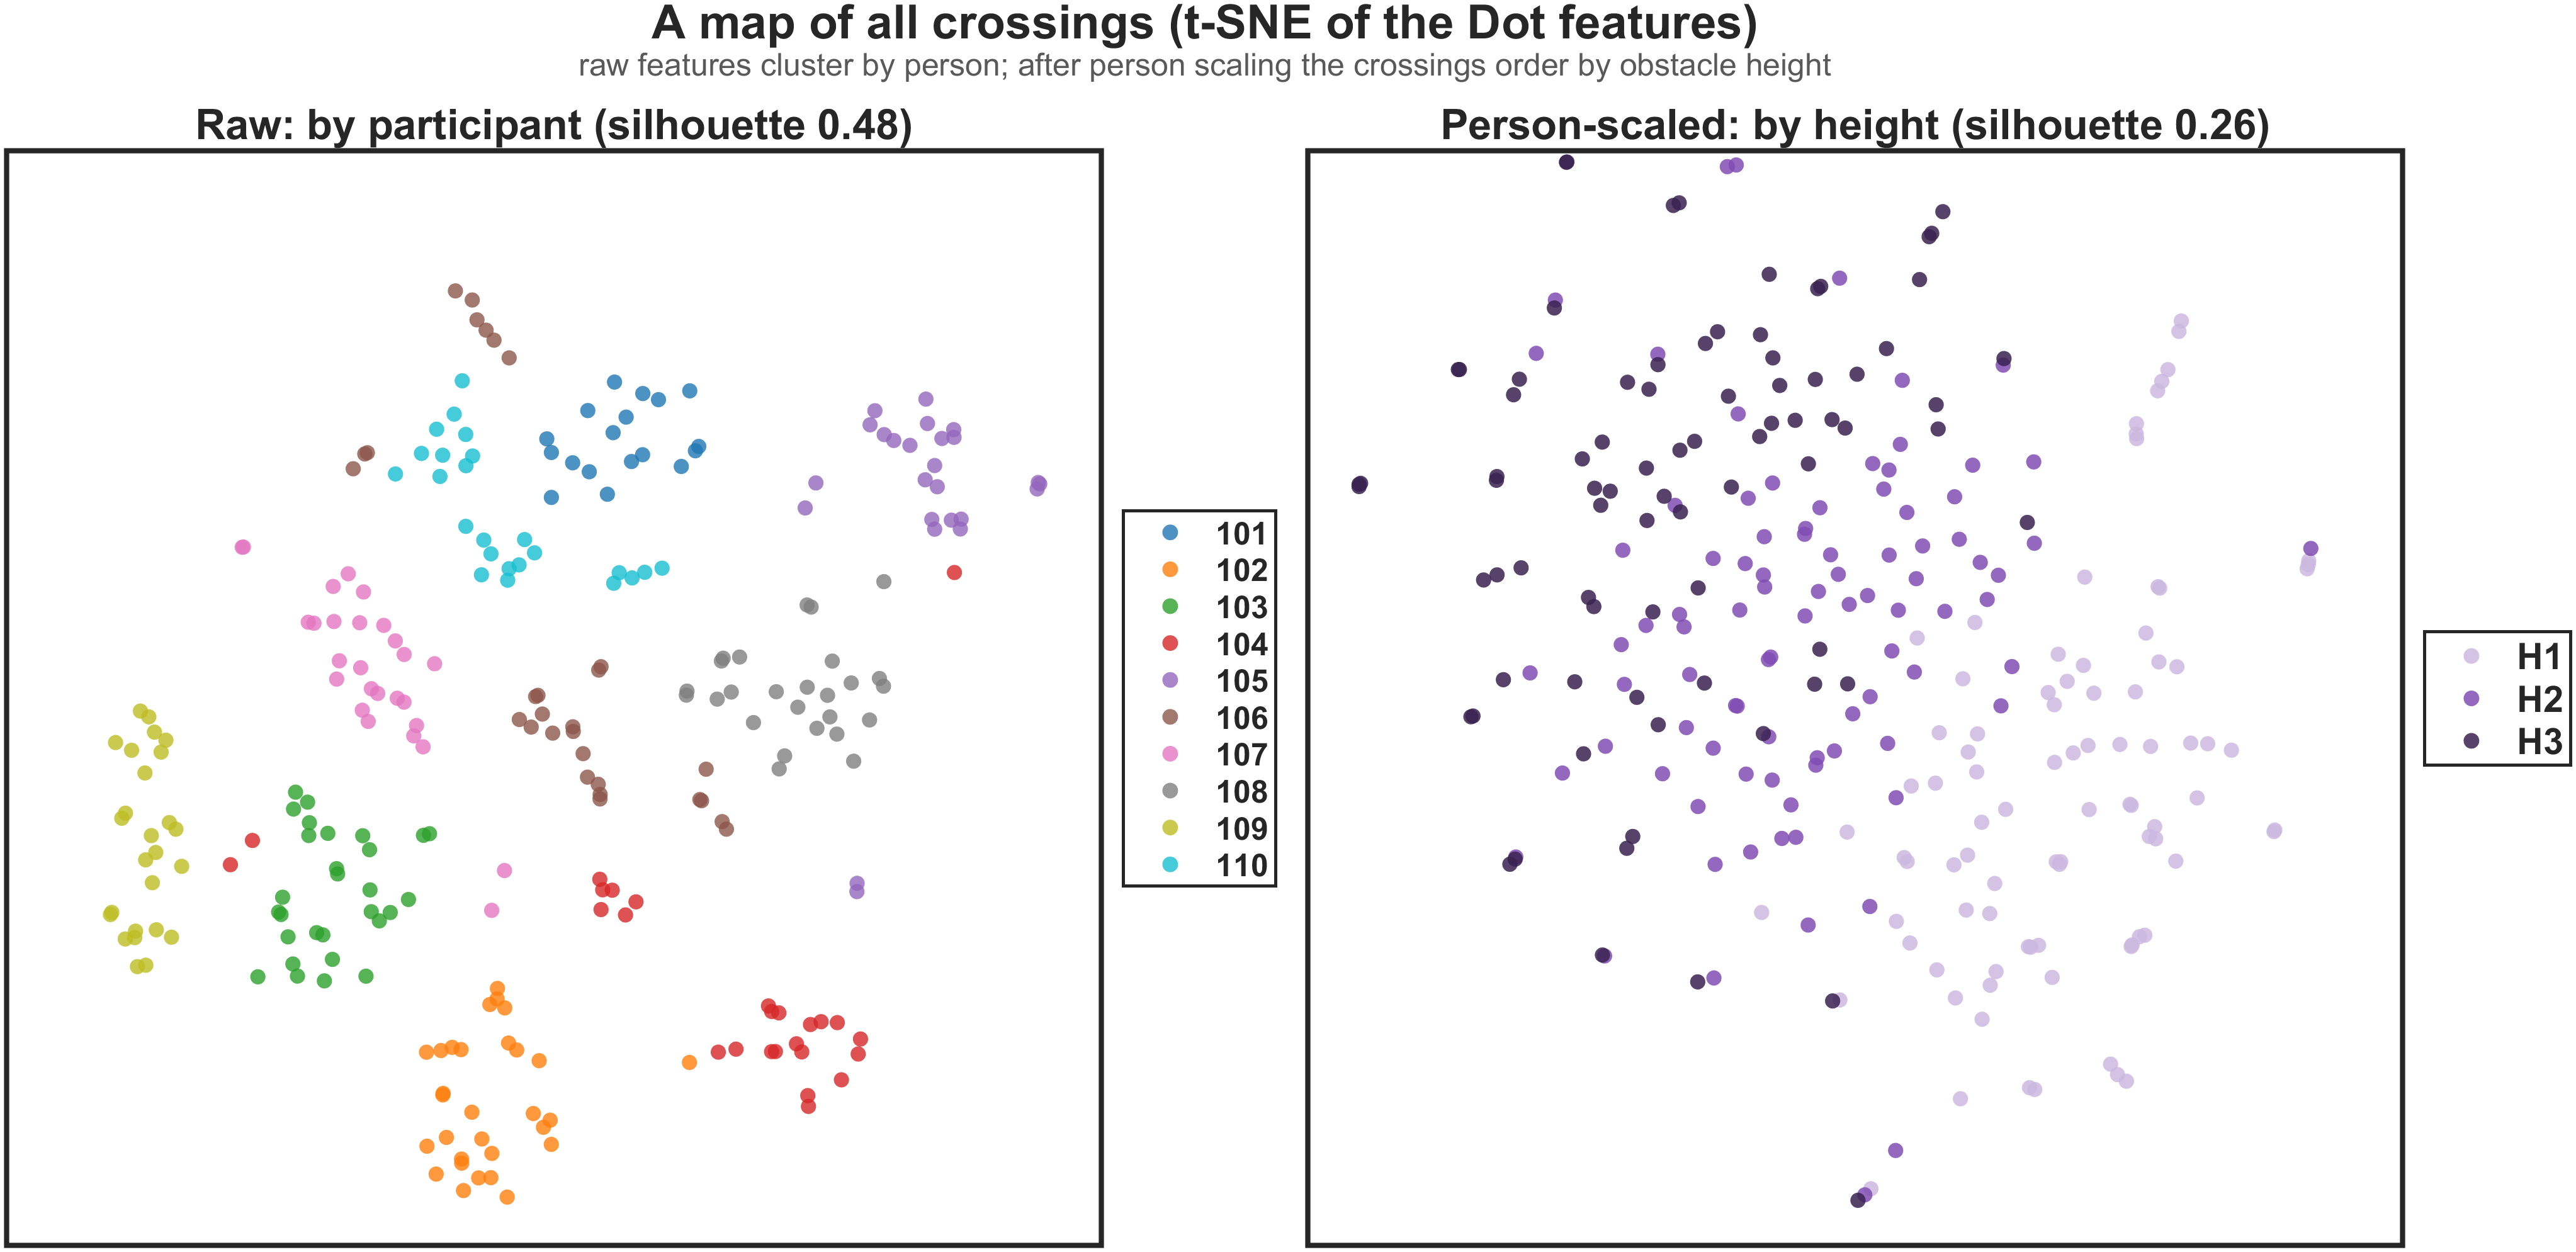
\includegraphics[width=\textwidth]{fig_story_embed.png}
\caption{t-SNE map of all crossings. Left: raw features coloured by participant. Right: person-scaled features coloured by
obstacle height (light to dark = H1 to H3). Silhouette (separation of the groups, $-1$ to 1) in the panel titles.}
\label{fig:embed}
\end{figure}

\subsubsection{The personal obstacle margin}

Per participant, the foot lift predicted by their own dose-response line at the cohort's mean obstacle height is their
``personal margin''. It differs between people by about two thirds of the step between neighbouring heights
(Table~\ref{tab:margin}: SD 64\,mm vs a 98\,mm step for the leading foot) and is barely predictable from the person's normal
walking ($r = 0.43$) or leg length ($r = 0.20$). An unseen person's margin therefore shifts every crossing toward a
neighbouring height, which caps generic models (Section~\ref{sec:res-height}).

\begin{table}[htbp]
\centering
\caption{Personal obstacle margin: spread across participants vs the step between heights.}
\label{tab:margin}
\begin{adjustbox}{max width=\textwidth}
{\footnotesize
\begin{tabular}{lrrrrr}
\toprule
\textbf{variable} & \textbf{between-person SD} & \textbf{step between heights} & \textbf{SD / step} & \textbf{r with level-walk value} & \textbf{r with leg length} \\
\midrule
lead foot lift & 64 mm & 98 mm & 0.66 & 0.43 & 0.20 \\
trail foot lift & 76 mm & 105 mm & 0.72 & $-$0.22 & 0.04 \\
\bottomrule
\end{tabular}
}
\end{adjustbox}

\end{table}

\subsubsection{The two legs}

The leading leg is not chosen by dominance: 45\,\% of the crossings were led with the dominant leg, and most participants
alternate (Table~\ref{tab:leads} in Appendix~\ref{app:extra}); the Dot recovers which leg leads in 100\,\% of the crossings
(Table~\ref{tab:leadtrail}). Within a crossing, once the shared obstacle effect is removed, the two legs vary independently
($\lvert r\rvert \leq 0.12$, Table~\ref{tab:coupling}): the leading leg tells how high the obstacle is, not whether the trailing
foot will under-lift on this crossing.

\begin{table}[htbp]
\centering
\caption{Coupling of the two legs: correlation of the crossing-to-crossing deviations from each participant $\times$ obstacle mean.}
\label{tab:coupling}
\begin{adjustbox}{max width=\textwidth}
{\footnotesize
\begin{tabular}{llr}
\toprule
\textbf{leading leg} & \textbf{trailing leg} & \textbf{r of the deviations} \\
\midrule
lead foot lift & trail foot lift & 0.11 \\
lead clearance (camera) & trail clearance (camera) & $-$0.12 \\
lead foot lift & trail clearance (camera) & $-$0.05 \\
lead thigh flexion & trail shank backward tilt & $-$0.07 \\
\bottomrule
\end{tabular}
}
\end{adjustbox}

\end{table}

\subsubsection{Does the camera confirm the scaling?}

The foot lift above is measured by the Dot foot sensor (on the top of the foot). The camera toe marker confirms the scaling but with a
smaller slope (Table~\ref{tab:validityslopes}): +8.8\,mm (leading) and +7.5\,mm (trailing) per cm of obstacle, against +10.1 and
+11.1\,mm for the sensor. The sensor rises more than the toe, especially on the trailing foot, which crosses heel-up. Crossing by
crossing (Table~\ref{tab:validityagree}), the sensor rise agrees well with the camera toe rise for the leading foot (bias +8\,mm,
$r = 0.82$, within person 0.90) and less for the trailing foot (bias +48\,mm, $r = 0.62$); the provisional rigid-body toe estimate
removes the trailing bias but not the scatter. Together with the flat clearance slope (Table~\ref{tab:lme}), people raise the toe by
slightly less than the obstacle height and accept a marginally smaller clearance for higher obstacles (not significant).

\begin{table}[htbp]
\centering
\caption{Foot lift per cm of obstacle measured by the camera toe marker and by the Dot (mixed model, 95\,\% CI).}
\label{tab:validityslopes}
\begin{adjustbox}{max width=\textwidth}
{\footnotesize
\begin{tabular}{lrr}
\toprule
\textbf{foot lift measure} & \textbf{leading limb, slope per cm (95\% CI)} & \textbf{trailing limb, slope per cm (95\% CI)} \\
\midrule
camera toe rise & +8.8 mm (+7.0 to +10.6) & +7.5 mm (+5.4 to +9.6) \\
IMU foot-sensor rise & +10.1 mm (+9.4 to +10.8) & +11.1 mm (+9.7 to +12.6) \\
IMU toe rise (rigid-body, provisional) & +10.1 mm (+9.4 to +10.8) & +10.5 mm (+9.1 to +11.8) \\
\bottomrule
\end{tabular}
}
\end{adjustbox}

\end{table}

\begin{table}[htbp]
\centering
\caption{Agreement of the Dot foot lift with the camera toe rise, per crossing (Bland--Altman bias, SD and 95\,\% limits; correlation
overall and within participant).}
\label{tab:validityagree}
\begin{adjustbox}{max width=\textwidth}
{\scriptsize
\begin{tabular}{llrrrrrrr}
\toprule
\textbf{IMU vs camera toe rise} & \textbf{limb} & \textbf{crossings} & \textbf{bias (mm)} & \textbf{SD (mm)} & \textbf{95\% limits (mm)} & \textbf{median abs. difference (mm)} & \textbf{r} & \textbf{within-person r (median)} \\
\midrule
IMU foot-sensor rise & lead & 260 & +8 & 66 & $-$122 to +137 & 30 & 0.82 & 0.90 \\
IMU foot-sensor rise & trail & 259 & +48 & 108 & $-$163 to +260 & 77 & 0.62 & 0.70 \\
IMU toe rise (rigid-body, provisional) & lead & 260 & +5 & 66 & $-$124 to +134 & 29 & 0.82 & 0.90 \\
IMU toe rise (rigid-body, provisional) & trail & 259 & $-$3 & 109 & $-$216 to +210 & 46 & 0.60 & 0.69 \\
\bottomrule
\end{tabular}
}
\end{adjustbox}

\end{table}

\subsubsection{No anticipation in the approach}

None of the variables available before the leading foot leaves the floor changes with obstacle height (Table~\ref{tab:anticipation}):
the two approach strides, the approach speed and the leading-foot stance all have slopes indistinguishable from zero and explain at
most 1\,\% of the within-person variance; the camera trailing-foot placement before the obstacle explains 4\,\%. The four IMU
approach variables classify the height at chance level (forest 41.6\,\%, logistic regression 30.8\,\%, permutation $p = 0.75$).
The adaptation to the obstacle height happens inside the crossing step itself, starting at the leading toe-off.

\begin{table}[htbp]
\centering
\caption{Anticipation: change per cm of obstacle of the variables before the crossing step (mixed model) and their within-person
$\eta^2$.}
\label{tab:anticipation}
\begin{adjustbox}{max width=\textwidth}
{\footnotesize
\begin{tabular}{p{6.2cm}rrrr}
\toprule
\textbf{variable} & \textbf{slope per cm} & \textbf{95\% CI} & \textbf{p} & \textbf{$\eta^2$ within person} \\
\midrule
stride two before the crossing stride (leading foot, mm) & $-$1.38 & $-$4.55 to +1.78 & 0.346 & 0.01 \\
stride just before the crossing stride (leading foot, mm) & +0.519 & $-$1.32 to +2.36 & 0.574 & 0.01 \\
approach speed (m/s) & $-$0.000239 & $-$0.00193 to +0.00145 & 0.752 & 0.01 \\
leading-foot stance before its crossing swing (s) & +0.000492 & $-$0.000593 to +0.00158 & 0.351 & 0.01 \\
trailing toe before the obstacle at its toe-off (camera, mm) & +3.29 & $-$3.64 to +10.2 & 0.312 & 0.04 \\
\bottomrule
\end{tabular}
}
\end{adjustbox}

\end{table}

